\documentclass{article}
\usepackage[utf8]{inputenc}
\usepackage{array}
\usepackage{wrapfig}
\usepackage{multirow}
\usepackage{tabu}
\usepackage{graphicx}

\title{Report}
\author{Tuğrul Tosun}

\begin{document}

\maketitle
\section{Part 1: Decision Tree}
\subsection{Information Gain}
Test result accuracy for information gain is 0.9490740740740741\\
You can find tree diagram in infogain.pdf file.
\subsection{Gain Ratio}
Test result accuracy for gain ratio is 0.9513888888888888\\
You can find tree diagram in gainratio.pdf file.
\subsection{Average Gini Index}
Test result accuracy for gain ratio is 0.9490740740740741\\
You can find tree diagram in avgginiindex.pdf file.
\subsection{Gain Ratio with Chi-squared Pre-pruning}
Test result accuracy for gain ratio with chi-squared\\
pre-pruning is 0.9502314814814815. You can find tree \\
diagram in gainratiopreprun.pdf file.
\subsection{Gain Ratio with Reduced Error Post-pruning}
Test results and referring to the tree diagram.

\vspace{20mm}
\maketitle
\section{Part 2: Support Vector Machine}
\subsection{First Part}
Small C values will result in a large margin at cost of misclassifying some data points.Large C values will 
result in narrow margin and makes constraints hard to ignore.\\

\begin{tabular}{c|c}
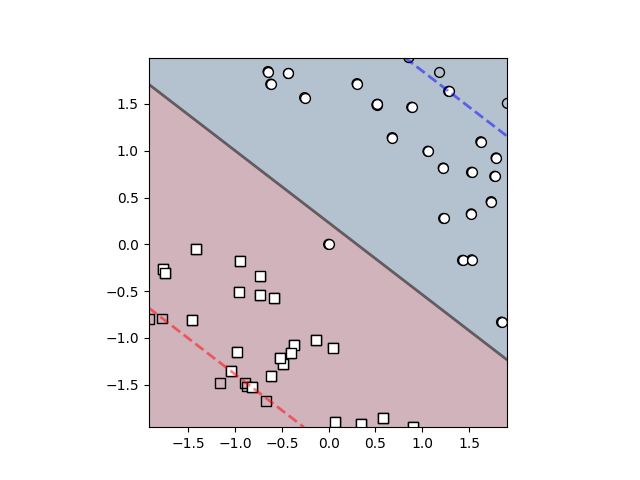
\includegraphics[scale=0.4]{hw3images/svmfirstpartc=0d01.png}&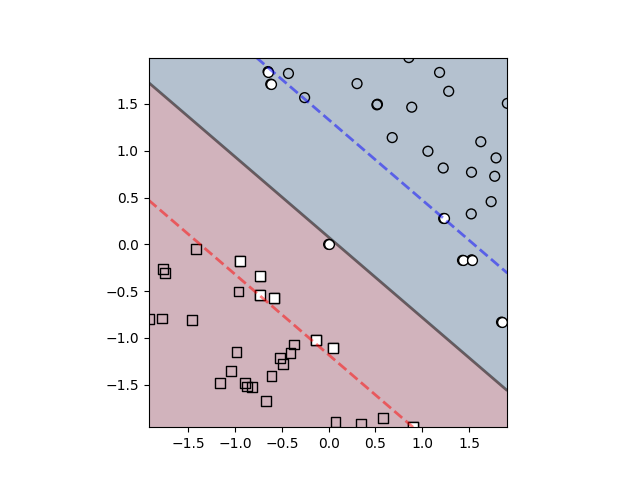
\includegraphics[scale=0.4]{hw3images/svmfirstpartc=0d1.png}\\
{svm first part C=0.01}&{svm first part C=0.1}\\
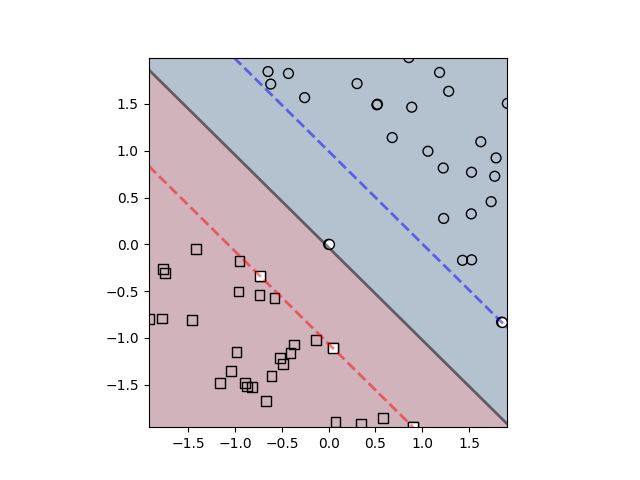
\includegraphics[scale=0.4]{hw3images/svmfirstpartc=1.png}&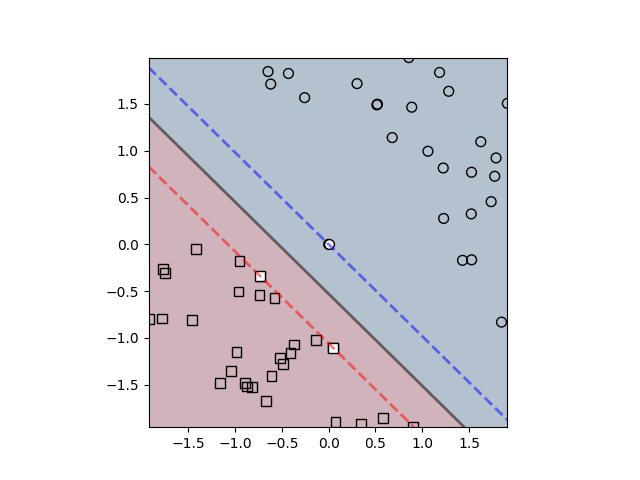
\includegraphics[scale=0.4]{hw3images/svmfirstpartc=10.png}\\
{svm first part C=1}&{svm first part C=10}\\
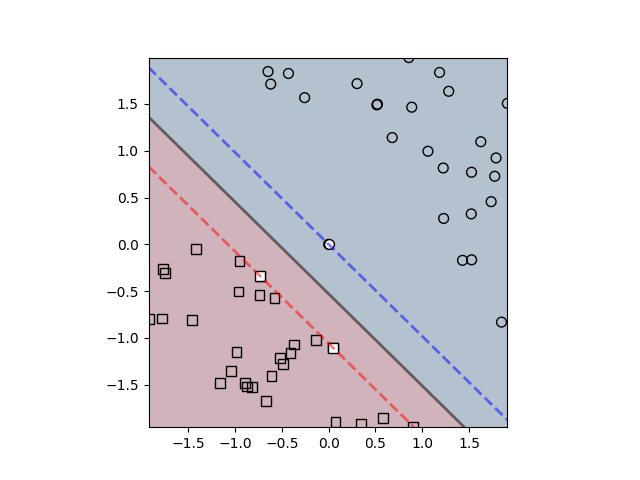
\includegraphics[scale=0.4]{hw3images/svmfirstpartc=100.png}&\\
{svm first part C=100}&\\
\end{tabular}
\subsection{Second Part}
Since data is not linearly seperable linear kernel is not suitable to our data.Rbf kernel was best for our data as it find better hyperplane that separate our data very well. Polynomial kernel separate our data from the point where density increased but was not successful on separating data well. Sigmoid kernel produced meaningless results on our data.\\
\begin{tabular}{c|c}
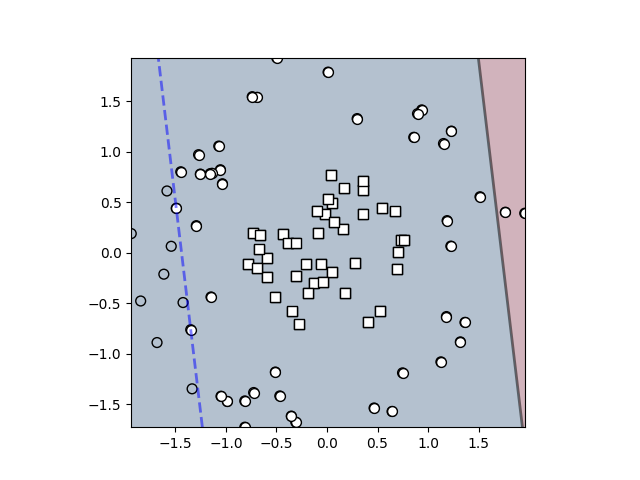
\includegraphics[scale=0.4]{hw3images/svmsecondarypartlinearkernel.png}&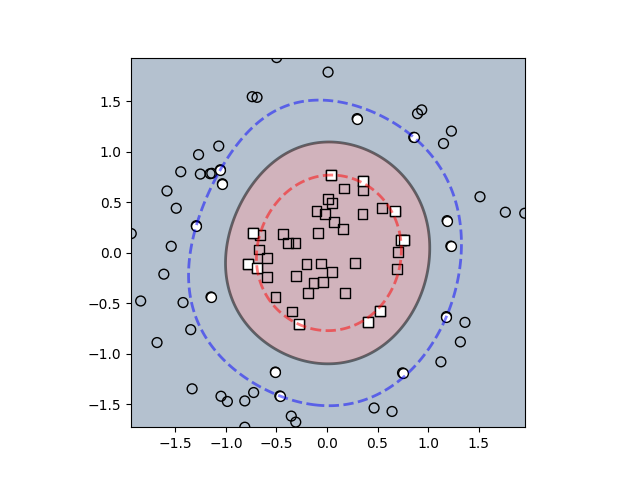
\includegraphics[scale=0.4]{hw3images/svmsecondarypartrbfkernel.png}\\
{svm second part linear kernel}&{svm second part rbf kernel}\\
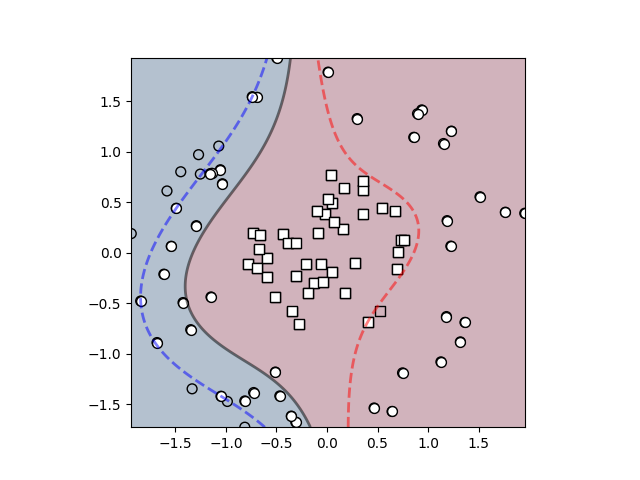
\includegraphics[scale=0.4]{hw3images/svmsecondarypartpolynomialkernel.png}&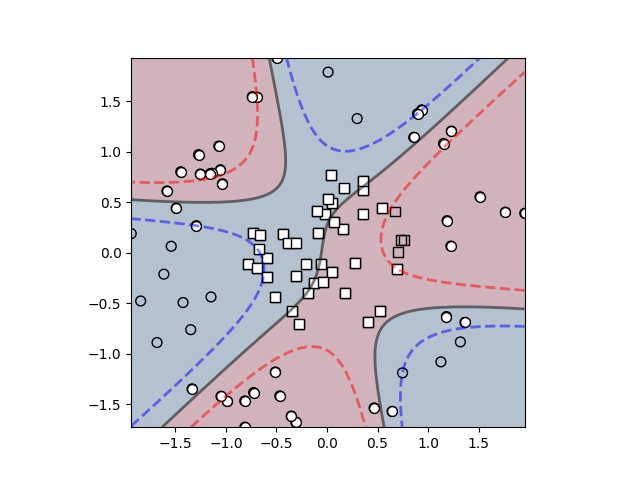
\includegraphics[scale=0.4]{hw3images/svmsecondarypartsigmoidkernel.png}\\
{svm second part poly kernel}&{svm second part sigmoid kernel}\\
\end{tabular}

\subsection{Third Part}
Best hyperparameters of model was kernel=rbf gamma=0.01 and C=10,100\\
My model gave 0.8095238095238095 accuracy on test data set.
\begin{table}[h]
    \centering
    \begin{tabular}{|c|c|c|c|c|c|c|c|}
    \hline
    \multirow{2}{5em}{gamma} & \multicolumn{5}{c|}{C} \\
        & 0.01 & 0.1 & 1 & 10 & 100 \\
        \hline \hline
        -  & 0.638 & 0.644 & 0.698 & 0.707 & 0.707 \\
        \hline
    \end{tabular}
    \caption{Linear kernel}
    \label{tab:linear}
\end{table}

\begin{table}[h]
    \centering
    \begin{tabular}{|c|c|c|c|c|c|c|c|}
    \hline
    \multirow{2}{5em}{gamma} & \multicolumn{5}{c|}{C} \\
        & 0.01 & 0.1 & 1 & 10 & 100 \\
        \hline \hline
        0.00001  & 0.538 & 0.538 & 0.538 & 0.564 & 0.627 \\
        0.0001  & 0.538 & 0.538 & 0.557 & 0.623 & 0.667 \\
        0.001  & 0.538 & 0.551 & 0.633 & 0.690 & 0.728 \\
        0.01  & 0.538 & 0.538 & 0.734 & 0.742 & 0.742 \\
        0.1  & 0.538 & 0.538 & 0.710 & 0.710 & 0.710 \\
        1  & 0.538 & 0.538 & 0.710 & 0.710 & 0.710 \\
        \hline
    \end{tabular}
    \caption{RBF kernel}
    \label{tab:rbf}
\end{table}

\begin{table}[h]
    \centering
    \begin{tabular}{|c|c|c|c|c|c|c|c|}
    \hline
    \multirow{2}{5em}{gamma} & \multicolumn{5}{c|}{C} \\
        & 0.01 & 0.1 & 1 & 10 & 100 \\
        \hline \hline
        0.00001  & 0.538 & 0.538 & 0.538 & 0.538 & 0.538 \\
        0.0001  & 0.538 & 0.538 & 0.538 & 0.538 & 0.562 \\
        0.001  & 0.538 & 0.561 & 0.612 & 0.692 & 0.731 \\
        0.01  & 0.692 & 0.731 & 0.731 & 0.727 & 0.727 \\
        0.1  & 0.727 & 0.727 & 0.727 & 0.727 & 0.727 \\
        1  & 0.727 & 0.727 & 0.727 & 0.727 & 0.727 \\
        \hline
    \end{tabular}
    \caption{Polynomial kernel}
    \label{tab:poly}
\end{table}

\begin{table}[!h]
    \centering
    \begin{tabular}{|c|c|c|c|c|c|c|c|}
    \hline
    \multirow{2}{5em}{gamma} & \multicolumn{5}{c|}{C} \\
        & 0.01 & 0.1 & 1 & 10 & 100 \\
        \hline \hline
        0.00001  & 0.538 & 0.538 & 0.539 & 0.539 & 0.609 \\
        0.0001  & 0.538 & 0.538 & 0.539 & 0.610 & 0.635 \\
        0.001  & 0.538 & 0.538 & 0.568 & 0.543 & 0.540 \\
        0.01  & 0.538 & 0.536 & 0.495 & 0.472 & 0.472 \\
        0.1  & 0.538 & 0.538 & 0.538 & 0.538 & 0.538 \\
        1  & 0.538 & 0.538 & 0.538 & 0.538 & 0.538 \\
        \hline
    \end{tabular}
    \caption{Sigmoid kernel}
    \label{tab:sigmoid}
\end{table}



\newpage
\subsection{Fourth part}
\subsubsection{Without handling the imbalance problem}
Accuracy result on test data is 0.8333333333333334.No,it can lead misunderstanding such as when dataset is imbalanced accuracy will be more dependent of dominant data.


\subsubsection{Oversampling the minority class}
Report your test accuracy, confusion matrix and comment on them.

\subsubsection{Undersampling the majority class}
Report your test accuracy, confusion matrix and comment on them.

\subsubsection{Setting the class\_weight to balanced}
Report your test accuracy, confusion matrix and comment on them.


\end{document}

